\documentclass{article}%
\usepackage[T1]{fontenc}%
\usepackage[utf8]{inputenc}%
\usepackage{lmodern}%
\usepackage{textcomp}%
\usepackage{lastpage}%
\usepackage[head=40pt,margin=0.5in,bottom=0.6in]{geometry}%
\usepackage{graphicx}%
%
\title{\textbf{Gobierno cede a China operaciones de Pdvsa y de las empresas básicas}}%
\author{ANA DÍAZ | anadiaz@el{-}nacional.com}%
\date{21/11/2018}%
%
\begin{document}%
\normalsize%
\maketitle%
\textbf{URL: }%
http://www.el{-}nacional.com/noticias/economia/gobierno{-}cede{-}china{-}operaciones{-}pdvsa{-}las{-}empresas{-}basicas\_260528\newline%
%
\textbf{Periodico: }%
EN, %
ID: %
260528, %
Seccion: %
Economía\newline%
%
\textbf{Palabras Claves: }%
NO\_TIENE\newline%
%
\textbf{Derecho: }%
CONTEXTO%
, Otros Derechos: %
2.3%
, Sub Derechos: %
2.3.1%
\newline%
%
\textbf{EP: }%
NO\newline%
\newline%
%
\textbf{\textit{Sindicalistas afirmaron que la decisión es parte del pago de la deuda externa con Pekín, en la que los asiáticos tienen las ventajas de mano de obra barata, energía y materias primas}}%
\newline%
\newline%
%
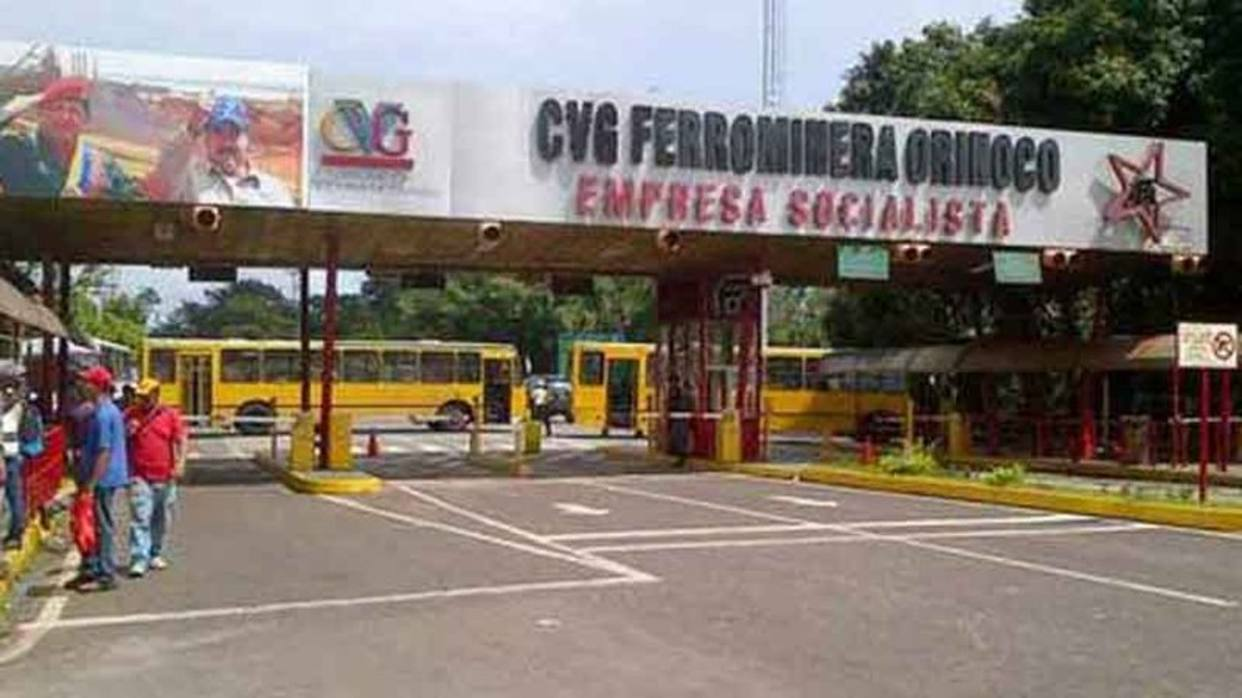
\includegraphics[width=300px]{219.jpg}%
\newline%
%
Los compromisos del gobierno para cancelar la deuda externa con China llevan a que el postulado nacionalista y estatista del socialismo del siglo XXI caiga en una fuerte contradicción. “El gobierno de Nicolás Maduro adelanta un plan agresivo de privatización de Petróleos de Venezuela y de las empresas básicas de Guayana con compañías chinas”, aseguró el sindicalista José Bodas, directivo de~la Federación~Única de Trabajadores Petroleros de Venezuela.%
\newline%
%
El sindicalista afirmó que “se trata de una privatización en la que las condiciones de la sociedad son más desventajosas para Venezuela, que tiene una posición de vendedor empobrecido frente al comprador”.%
\newline%
%
Precisó que en la empresa mixta Sinovensa, en~la faja~petrolífera~del Orinoco, la presión de los chinos condujo a que la participación accionaria de~la Corporación~Petrolera~Nacional China pasará recientemente de 40\% a 49,9\%, mientras que Pdvsa bajó de 60\% a 50,1\%. Ese esquema, agregó, se repetirá en otros negocios conjuntos con esa y otras firmas privadas del país asiático.%
\newline%
%
Desde hace un par de semanas, los sindicatos y trabajadores de las empresas básicas de~la Corporación Venezolana~de Guayana han presenciado reuniones de empresarios chinos con sus directivos, especialmente en~la Ferrominera~del Orinoco.%
\newline%
%
“En Ferrominera hubo una reunión en la que los chinos manifestaron que aportarán 970 millones de dólares para recuperar y administrar las operaciones de toda la cadena –extracción, pellas y briquetas– del mineral de hierro”, señaló Rubén González, presidente del sindicato de la empresa, y enfatizó: “Es traición a la patria la entrega a los chinos de Ferrominera y de las otras empresas básicas. El gobierno las llevó al caos porque no las supo administrar, dilapidó los dividendos generados y no hizo las inversiones necesarias para mantener las operaciones de manera eficiente”.%
\newline%
%
González insistió en que “los 7.000 trabajadores de Ferrominera no necesitan a los chinos”, pues han demostrado que tienen la capacidad para hacer productiva la compañía que registró en el pasado producciones récord de 22 millones de toneladas al año.%
\newline%
%
Desde hace un año y cuatro meses las operaciones de la extractora de hierro y de Bauxilum están totalmente paralizadas, mientras que~la Siderúrgica~del Orinoco, Venalum y Alcasa operan a 20\%, 25\% y 15\% de su capacidad instalada, añadió el sindicalista.%
\newline%
%
Profesionales Unidos por Ferrominera alertó en un comunicado que el gobierno entrega esa empresa a consorcios chinos, además de Bauxilum, Alcasa y Venalum, filiales del aluminio de~la CVG.%
\newline%
%
Indica que si la privatización contribuye a la recuperación y mejora de las industrias de CVG y las condiciones de trabajo del personal, es bienvenida. No obstante, advierte: “El problema es que las empresas que negociaron con el régimen ya tienen antecedentes de obras sin terminar y miles de millones de dólares perdidos”.%
\newline%
%
Yunis Hernández, dirigente sindical de Sidor, señaló que la presencia de los chinos preocupa a los trabajadores de las empresas básicas, quienes tienen la certeza de que las últimas decisiones salariales y de aplanamiento de los tabuladores tomadas por el gobierno son para atraer las inversiones de China y poner a producir las plantas.%
\newline%
%
“En Venezuela y en muchos países se sabe que los chinos no son los mejores patronos, pero ya el gobierno de Maduro les allana el terreno en la oferta de su paquete de cesión de las empresas que incluye como ventajas mano de obra demasiado barata, energía abundante y materias primas como petróleo, aluminio y hierro”, expresó Bodas.%
\newline%
%
La Cifra%
\newline%
%
22 millones de toneladas de mineral de hierro fue la producción récord de~~Ferrominera del Orinoco en 2006. Desde hace un año y cuatro meses la empresa está paralizada%
\newline%
%
\end{document}